% latex article template

% cheat sheet(eng): http://www.pvv.ntnu.no/~walle/latex/dokumentasjon/latexsheet.pdf
% cheat sheet2(eng): http://www.pvv.ntnu.no/~walle/latex/dokumentasjon/LaTeX-cheat-sheet.pdf
% reference manual(eng): http://ctan.uib.no/info/latex2e-help-texinfo/latex2e.html

% The document class defines the type of document. Presentation, article, letter, etc. 
\documentclass[12pt, a4paper]{article}

% packages to be used. needed to use images and such things. 
\usepackage[pdfborder=0 0 0]{hyperref}
\usepackage[utf8]{inputenc}
\usepackage[english]{babel}
\usepackage{graphicx}
\PassOptionsToPackage{hyphens}{url}

% hides the section numbering. 
\setcounter{secnumdepth}{-1}

% Graphics/image lications and extensions. 
\DeclareGraphicsExtensions{.pdf, .png, .jpg, .jpeg}
\graphicspath{{./images/}}

% Title or header for the document. 
\title{
	TIØ4116, Exercise 8. 
}
% Author
\author{
	Magnus L. Kirø \\
}
\date{\today}

\begin{document}
\maketitle
\pagenumbering{arabic}

\section{Task 1}

\paragraph{A}
In the long run the price will be 18p, because the 3600 factor will be so small
that it will not matter. 

At the same time we will have an excellent director that earns a minimum of 30\% more than
the average director. Based on the cost difference. Costs of the two: 25/36~=0.7
vs 1, giving cost difference of 30\%. 

\paragraph{B}
The market turnover is described by p*q which gives us (25/36)*1000\^2 *
18*1000, given that q and p are measurements of 1000NOK. This gives us a market
turnover of 1.25*10\^10 for the excellent directors, while the average will have
a turnover of 1.8*10\^10. By expecting that both types of directors have a
competitive market price we can assume that the excellent director earns the
difference in turnover as profit, resulting in an additional profit of
5.5*10\^9. 

\paragraph{C}
If all companies will tend towards hiring the more extraordinary directors the
annual wages will move toward a 30\% difference. 


\section{Task 2}
\paragraph{A}
Given q=1 we have a market quantity of 505. With one production line we have
q=Q, giving us p=595. Profit is then p-q=90. This gives a gross margin of
90/505=17.8\%

\paragraph{B}
Given the addition of another production line we get: 
Cost=520, Price=590, Profit=70, gross margin=13.4\%.

\paragraph{C}
The maximum of profitable production lines are 3. 
This gives: cost=545, price=585, profit=40, and gross margin=3.7\%

See figure 1 for the graph plot of the cost and price functions. 

% image example. 
\begin{figure}[htb]
    \centering
    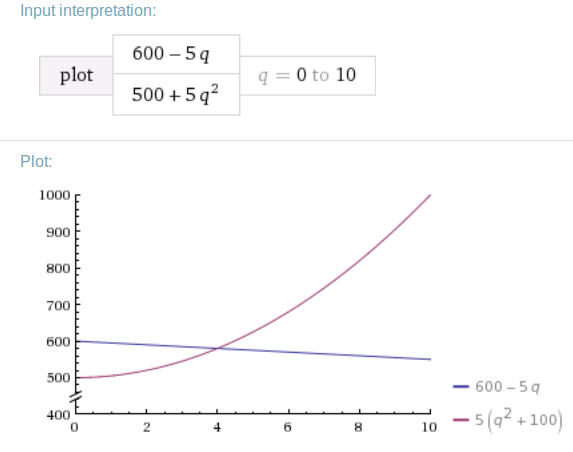
\includegraphics[width=\textwidth]{plot}
    \label{fig:plot}
    \caption{}
The graph show the price and cost function. The two graphs intersect at x=4,
which is the point where the profit if 0. 
\end{figure}

\paragraph{D}
Given the production lines n, we have the return to scale function as 10n+10.
This describes the decrease in profit as we increase production with lowered
sales prices. We can see this development from previous calculations which
gives us profit by production lines: n=1 - profit=90, n=2 - profit=70, n=3 -
profit=40, and n=4 - profit=0. 

\section{Task 3}
\paragraph{A}
The expression for cost is: 4sqrt(2)r+6r. By looking at the initial function
one could indicate that the function is linear. The marginal cost is: 11.66. The
average cost is: (total cost / quantity), as the quantity is not given in
this case we cannot calculate the average cost.

\paragraph{B}
% image example. 
\begin{figure}[htb]
    \centering
    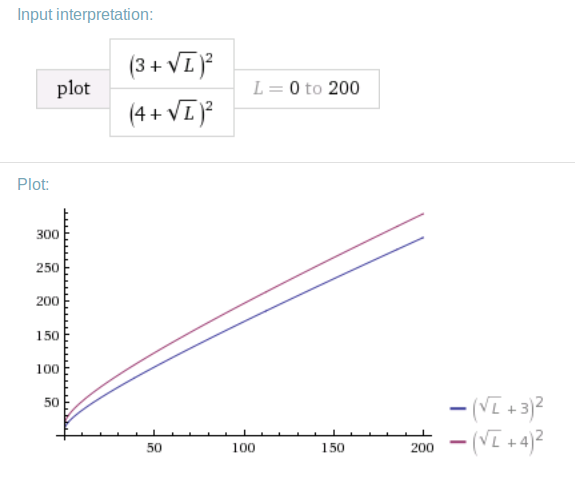
\includegraphics[width=\textwidth]{plot2}
    \label{fig:plot2}
    \caption{}
The graphs shows the cost function of the two factories. The two functions are
near linear and becomes more linear as the values increases. 
\end{figure}
The two factories have equal profit margin per quantity, but one factory has
bigger production capacity than the other, which increases the production cost. 

\paragraph{C}
The factories would divide the work load with 64\% of the load to the bigger
factory and 36\% to the smaller. 
The marginal value can be found by letting the quantity be 1. Then we get the
marginal value to be 41.

\section{task 4}


\end{document}
This is never printed
